\begin{song}{Divoké koně}{C}{Jaromír Nohavica}

\begin{SBVerse}

$|$: \Ch{ami}{Já }viděl \Ch{dmi}{divo}ké \Ch{ami}{koně}, \Ch{C}{běž}eli \Ch{dmi}{soum}ra\Ch{ami}{kem, }:$|$

\Ch{dmi}{Vzduch} \Ch{ami}{těžký} \Ch{dmi}{byl }a divně \Ch{ami}{voněl} \Ch{Ddmi}{tabá--}\Ch{F}{kem.}

\Ch{dmi}{Vzduch} \Ch{ami}{těžký} \Ch{dmi}{byl} a divně \Ch{ami}{voněl} \Ch{E7}{tabá}\Ch{ami}{kem}.

\end{SBVerse}

\begin{SBVerse}
$|$: Běželi, běžěli, bez uzdy a sedla, krajinou řek a hor, :$|$

$|$: Sper to čert, jaká touha je to vedla za obzor. :$|$
\end{SBVerse}

\begin{SBVerse}

$|$: Snad vesmír nad vesmírem, snad lístek na věčnost, :$|$

$|$: naše touho ještě neumírej, sil máme dost. :$|$

\end{SBVerse}

\begin{SBVerse}
$|$: V nozdrách sládne zápach klisen na břehu jezera, :$|$

$|$: milování je divoká píseň večera. :$|$
\end{SBVerse}

\begin{SBVerse}
$|$: Stébla trávy sklání hlavu , staví se do šiku, :$|$

$|$: král s dvořany přijíždí na popravu zbojníků. :$|$
\end{SBVerse}

\begin{SBVerse}
$|$: Chtěl bych jak divoký kůň běžet běžet, nemyslet na návrat, :$|$

$|$: s koňskými handlíři vyrazit dveře, to bych rád. :$|$
\end{SBVerse}

\begin{SBVerse}
Já viděl divoké koně\dots
\end{SBVerse}
\begin{center}
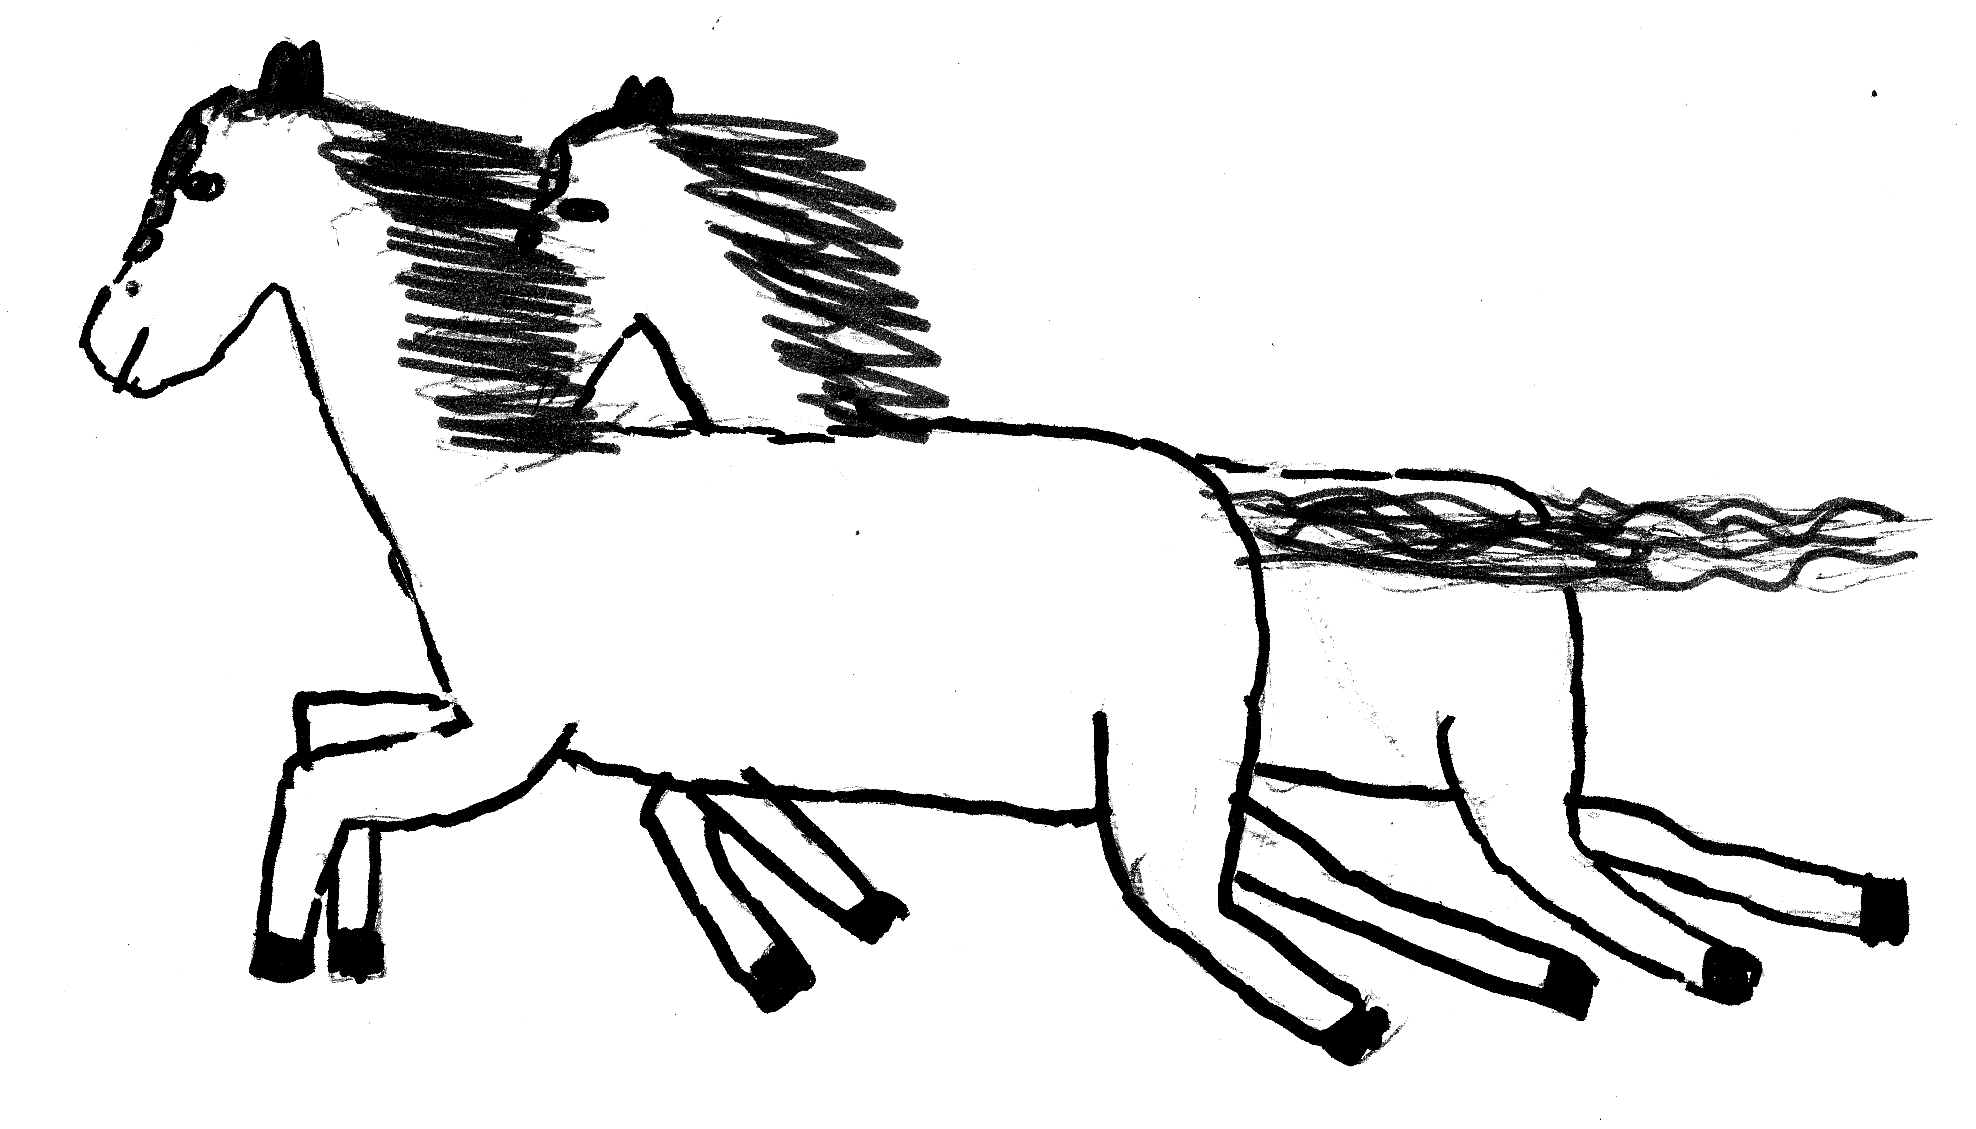
\includegraphics[width=5cm]{pict/divoci_kone}
\end{center}
\end{song}

\pagebreak